\documentclass{article}

\usepackage[a4paper, portrait, margin=1.5cm]{geometry}

\usepackage{fancyhdr}
\usepackage{hyperref}
\setlength{\headheight}{15pt}

\usepackage[table]{xcolor}
%\usepackage{minipage}
\usepackage{float}
\usepackage{svg}
\usepackage{ltablex}

\setlength{\arrayrulewidth}{0.2mm}

\usepackage{tikz}
\usetikzlibrary{shapes, arrows.meta, positioning}

\usepackage{textcomp}
\usepackage{amsmath}
\usepackage{amsfonts}
\usepackage{amssymb}
\usepackage{mathrsfs}
\usepackage{mathtools}
\usepackage{cases}
\usepackage{siunitx}
\usepackage{gnuplottex}

\usepackage{multicol}

\usepackage{caption, booktabs}
\usepackage{caption}
\usepackage{subcaption}

\usepackage{csvsimple}
\usepackage{minted}
%\usepackage{xpatch}
\definecolor{light_grey}{gray}{0.9}
\setminted{frame=lines, framesep=2mm, bgcolor=light_grey, fontsize=\footnotesize, linenos}

\usepackage{algorithm}
\usepackage{algpseudocode}

\algdef{SE}[FOR]{For}{EndFor}[2]{\algorithmicfor\text{ }  #1 \textbf{to} #2 \algorithmicdo}{\algorithmicend\ \algorithmicfor}%

\usepackage{hyperref}
\hypersetup{colorlinks, citecolor=black, filecolor=black, linkcolor=black, urlcolor=black}

\title{CAB401 Project}
\author{Oliver Strong n11037580}
\date{\today}

\begin{document}

\maketitle
\tableofcontents
%\listofalgorithms
\section{Introduction}
This report will detail the process of parallelising a serial application, and the results of this process.
The original application is a C program that reads in any number of files and performs a byte pair encoding process.

\section{Original Application}
The application is a procedural program with a simple command line interface to control it. It has two modes, both train and status.
The train mode takes a project name, target vocabulary size, output filepath, and a n-long list of filepaths to train on. The status mode
can take a filepath to the output file and will print the vocabulary to stdout as JSON from which the 
status of the training can be determined.

The call graph of the application was generated by Doxygen and dot and is shown below.
\begin{figure}[H]
    \centering
    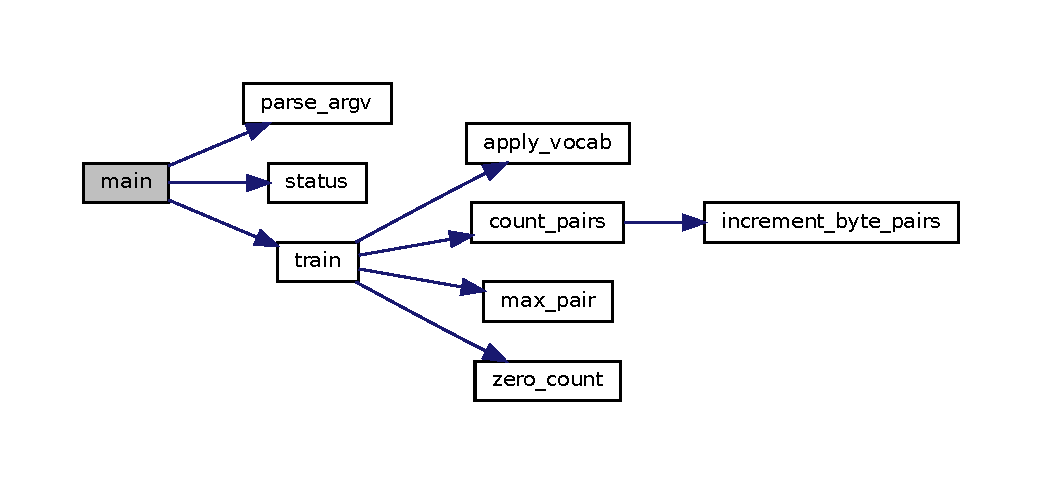
\includegraphics[width=0.6\textwidth]{original_application_callgraph.pdf}
    \caption{Call graph of the original application}
\end{figure}

The general algorithm of the original application is as follows

\begin{algorithm}[H]
    \caption{Original Application(mode, projectName, vocabSize, outputFilepath, inputFilepaths$[..N]$)} \label{alg:original}
    \textbackslash \textbackslash Input: String \textit{mode} which is either train or vocab, String \textit{projectName}, Natural number \textit{vocabSize}\\
    \textbackslash \textbackslash \hspace{1cm} String outputFilepath, many strings inputFilepaths that is \textit{N} long \\
    \textbackslash \textbackslash Output: File \textit{outputFilepath} with the vocabulary 
    \begin{algorithmic}[1]
        \State $vocabulary \gets \{\}$
        \If{mode == train}
            \For{$i\gets 0$}{$vocabLength$}
                \State $pairCounts \gets \{\}$
                \For{$j\gets 0$}{$N$}
                    \State $file \gets inputFilepaths[j]$
                    \State $buff \gets Read(file)$
                    \State $buff \gets transform(vocabulary, buff)$ 
                    \State $pairCounts \gets pairCounts \cup \text{countPairs}(buff)$
                \EndFor
                \State $vocabulary \gets vocabulary \cup \text{mostCommon}(pairCounts)$
                \State $outputFilepath \gets vocabulary$
            \EndFor
        \ElsIf{mode == status}
            \State $stdout \gets JSON(vocabulary)$
        \EndIf
    \end{algorithmic}
\end{algorithm}

If called with the command \mintinline{bash}{./train_vocab train project 260 output.vocab main.c} then the 
program will create a file called \textit{output.vocab} that contains the vocabulary of the files \textit{main.c}.
There will be a list of four replacements which are the most common byte pairs where each is recursively replaced from the 
start of the list. As main.c is a C file it will contain common pairs found in C source code. You can expect that the first replacement made 
will be $(32,32)$ to $256$ as $32$ is the ASCII code for a space character. If the author of the code
used four spaces for the indentation then the next most common pair will be $(256,256)$ which will be replaced with $257$.
 as the four 32's will have been replaced  with two 256's and then that will be replaced with a 257.


This vocabulary output can then be loaded at a later stage after being trained and used to encode 
some file you wish to feed into a language model.

A typical use case for this type of application is to take a large dataset, potentially multiple terrabytes of
data and use it to train a vocabulary so some statistical model can be fitted on the encoded data. 
This technique allows the model to see a more uniform distribution of token values as performing
token level predictions on unencoded data would lead to it overfitting on the most common tokens.

\section{Potential Parallelism}
From algorithm \ref{alg:original} the vocabulary is a 
flow, output, and anti dependence with the loop from \textit{i} to \textit{vocabLength}. This is
because the vocabulary starts empty and is built up on each iteration. This requires the previous 
iteration's value to be available so the files can be correctly transformed which is a flow dependence.
Then when the vocabulary is updated in each iteration it is an output dependence, and then in subsequent
iterations the vocabulary is used to transform the files which is later overwritten when it is updated, which is an anti dependence.

As the nature of the algorithm is to build up the vocabulary in a loop, it is not possible to parallelise the outer loop. 
This makes the inner loop the first candidate for parallelisation. The inner loop is a loop over the files that are to be trained on.
The original application is designed to preserve memory so on every iteration of the inner loop in algorithm \ref{alg:original}, 
the file is read into memory, and then transformed. This makes sure it is in a state that matches the current point of training.
These files could be processed in parallel, however, this would give too rough of a granularity which is not desirable. 
If parallelising at the file level, the program could have to wait on very large files to be processed 
causing other threads to wait excessively for synchronisation. This would lead to poor utilisation of the available compute if the files are 
inbalanced in size regardless of how the data is mapped to compute.

Given the predicted poor load balance of the file level parallelism, the operations that the loop performs
were investigated. 

\subsection{Byte pair tokeniser transform}
To perform the transformation there are two nested loops as per the following algorithm

\begin{algorithm}[H]
    \caption{Transform(vocabulary, buff)} \label{alg:transform}
    \textbackslash \textbackslash Input: Array of vocab \textit{vocabulary}, Array of symbols \textit{buff} \\
    \textbackslash \textbackslash Output: Array of symbols \textit{buff} with byte pairs replaced
    \begin{algorithmic}[1]
        \For{$i\gets 0$}{$len(vocabulary)$}
            \For{$j\gets 0$}{$len(buff)$}
                \If{$\text{buff}[i] == \text{SKIP\_TOKEN}$}
                    \State \textbf{continue}
                \EndIf
                \If{$\text{buff}[i] == \text{vocabulary}[j].b1$}
                    \State $p \gets 1$
                    \While{$j + p < len(buff)$}
                        \If{$\text{buff}[j+p] \neq \text{SKIP\_TOKEN}$}
                            \State \textbf{break}
                        \EndIf
                        \State $p \gets p + 1$
                    \EndWhile 
                    \If{$\text{buff}[i+1] == \text{vocabulary}[j].b2$}
                        \State $\text{buff}[i] \gets \text{vocabulary}[j].rep$
                        \State $\text{buff}[i+1] \gets \text{SKIP\_TOKEN}$
                    \EndIf
                    \State $j \gets j + p$
                \EndIf
            \EndFor
        \EndFor
    \end{algorithmic}    
\end{algorithm}

From algorithm \ref{alg:transform} it can be seen that the inner loop and outer loops both have 
flow and anti dependences. This makes the algorithm unsuitable for parallelisation. This means for this algorithm, applying
it to many files in parallel is the only suitable option.

\newpage
\subsection{Counting byte pairs}

The algorithm for counting byte pairs is as follows

\begin{algorithm}[H]
    \caption{CountPairs(buff)} \label{alg:countpairs}
    \textbackslash \textbackslash Input: Array of symbols \textit{buff} \\
    \textbackslash \textbackslash Output: Array of array of numbers \textit{pairCounts}
    \begin{algorithmic}[1]
        \State $pairCounts \gets \{\}$
        \For{$i\gets 0$}{$len(buff)$}
            \If{$\text{buff}[i] == \text{SKIP\_TOKEN}$}
                \State \textbf{continue}
            \EndIf
            \State $p \gets 1$
            \While{$i + p < len(buff)$}
                \If{$\text{buff}[i+p] \neq \text{SKIP\_TOKEN}$}
                    \State \textbf{break}
                \EndIf
                \State $p \gets p + 1$ 
            \EndWhile
            \If{$i + p == len(buff)$}
                \State $\text{return} {}$
            \EndIf

            \State $b_1 \gets buff[i]$
            \State $b_2 \gets buff[i+p]$
            \State $pair[b_1][b_2] \gets pair[b_1][b_2] + 1$
        \EndFor
    \end{algorithmic}
\end{algorithm}

In the algorithm it can be seen that there is a flow and anti dependence in the loop.
As the only dependence is the pair array, it is classed as a reduction operation.
The reduction operation in this algorithm is non trivial, as when indexing the pair there are 
possible branches and memory allocations that could be performed. This makes OpenMP's reduction clause
unsuitable for this operation. This would require a custom reduction operation to be implemented.

\subsection{The Clean Slate}

If the application is written from scratch and the parallelism available in the existing application is not
binding then through significant refactoring, the application could be made to be more parallelisable.

\subsubsection{Dealing with data in chunks}
It was discussed earlier that the file level parallelism would be too rough of a granularity to be useful.
However if "files" were to be replaced with "chunks" then the granularity would be more fine grained. The chunk
can have a size that is controlled by the programmer and can be adjusted to suit the data being processed.

The tokenisation step has to be performed on a file in its entirety as the byte pairs may span the 
chunk boundary. The ghost cell pattern will not help here because out of sequence tranformation of the chunk's 
underlying memory would lead to incorrect results. This means the tokenisation step has to be performed on 
each iteration, before creating the chunked views of the data that can have the byte pair counting 
performed on them. 

This improves load balance as the chunks can be distributed to the threads in a more balanced manner, however the
tokenisation step could still potentially be poorly balanced. This lead to the choice behind the methods of 
mapping the computation to the processors.

\section{Mapping computation to processors}
A number of tools were considered for the parallelisation of the application. The first tool considered was OpenMP.
OpenMP could be used to parallelise the loops using the \mintinline{c}{#pragma omp parallel for} directive. 
This would greatly simplify the implementation process, however it would also leave performance on the table.

As found in the GCC implementation of OpenMP the work is divided to threads in an unequal manner\ref{gcc_omp}.
As $\frac{1}{n}$ of the iterations are provided to the next free thread, the first thread ends up with most of the work.
This is not ideal, particularly if the file paths are delivered to the program in a descending order of file size.
This would lead to many threads stalling while the program waits on all threads to finish.

The next tool considered was POSIX pthreads. This would allow for a more fine grained control over the work 
division. A thread pool construct was built from scratch to manage the threads. The thread pool took a function pointer
and a void pointer to the function argument from a hand made thread safe FIFO queue implementation. 
When a thread was free it pulled the next task from queue. This ensured that if a thread was free it would 
always be able to request more work.

This meant that if there was no requirement for synchronisation between different tasks then the next task could 
be added to the queue so the pool could initiate work on it without delaying for synchronisation.


\subsection{Queue class implementation}
The queue was implemented as a circular buffer, which was an array of pointers with a mutex and two semaphores. One semaphore signaled when 
the queue had space to add a new element, and the other signaled when the queue was non empty. The mutex was used
to protect the indicies of the circular buffer from being modified by multiple threads at once.

The implementation of the queue resulted in a very small memory footprint. This meant that the queue was 
fast to access and modify.

\subsection{ThreadPool class implementation}
The threadpool was implemented as a class that took a number of desired threads in the constructor and launched
each thread to a function in the class. This \mintinline{C}{ThreadPool::start(void *arg)} function allowed the
thread to pull tasks from the threadsafe queue and execute them.

The class also implemented a destructor to join all the threads and free the memory used by the threads, abiding
by the RAII principle.


\section{Timing and profiling}

\section{Serial application profiling and analysis}
An analysis of the serial application is useful to determine the possible speedups due to 
parallelisation. 

%\begin{figure}[H]
%    \centering
%    \includegraphics[width=0.6\textwidth]{serial_summary.svg}
%    \caption{Timing analysis of the serial application}
%\end{figure}

From the figure it can be seen that there is a lot of time spent during the transform step. This is 
due to the fact that for every file the application receives, it reads it and transforms it \textit{n} 
(where \textit{n} is the length of the vocabulary in that iteration) so it is ready to have statistics
calculated. This is expensive as the algorithm has a quadtratic time complexity (with respect to the 
vocabulary size). The algorithm can be improved to have a linear time complexity by storing the 
transformed files in memory and only performing one step per statistics calculation iteration.

The analysis also shows that count\_pairs is a significant target for optimisation, which can be 
acheived with the thread pool.

This brings us 


An initial experiment was conducted to rewrite the entire serial application in a parallel manner using 
the structures and technologies discussed. Due to the limitation of the previous serial implementation 
there was a practical limit to the size of the vocabulary that could be trained. Due to the CPU time 
and memory tradeoff the vocabulary size was limited to 285, this would lead to both implementations 
counting and replacing the 30 most common byte pairs.

\begin{table}[H]
    \centering
    \begin{tabular}{|c|c|c|}
        \hline
        \textbf{Implementation} & \textbf{Time (s)} & \textbf{Peak Memory (MB)} \\        
        \hline
    \end{tabular}
\end{table}

\section{Testing of logical equivalence}

To make sure the implementations were logically equivalent, a short python script was written.

\begin{minted}{python}
parallel_filepath = open("parallel.vocab", "rb")
serial_filepath = open("serial.vocab", "rb")

parallel_output = parallel_filepath.read()
serial_output = serial_filepath.read()

if parallel_output == serial_output:
    print("The two implementations are equivalent")
else:
    print("The two implementations are not equivalent")
\end{minted}

This makes sure that each bite is the same in both files. This will only work where the same command 
is used to invoke both implementations.

The result of this test shows that the two implementations are equivalent. You can also see this by using 
the \textit{status} mode of the application to print the vocabulary as JSON.

\section{Tools used}

To compile the parallel application GCC-12 was used with the -O3, -fopenmp, and -lpthread flags. When debugging 
the application the \textit{strace} tool was particularly helpful. This allowed insight into the system calls that
the application was making. This was useful to determine why particular threads were going to sleep or not grabbing
work from the queue. \textit{-fsanatize=address} and valgrind were also invaluable in finding memory related bugs in the program.
There were instances where race conditions occured, particularly use after free bugs due to destructors being called
on data before threads had finished using it.

Orbit and perf were initially tried to profile the application, however Orbit did not provide sufficient
information regarding semaphore waiting times, cache misses, and other useful information. Perf was also 
tried, while it was very powerful it lacked the visualisation tools that Intel Advisor provided.

Intel Advisor was then used to profile the application. The roofline analysis was particularly useful to determine 
which loops were worth optimising further and which were not.

To perform the parllelisation of the application pthreads was used for multiprocessor parallelism and 
OpenMP was used for SIMD parallelism. 


\section{Process and Problems encountered}

\subsection{Initial experimentation}
The initial experiment involved using OpenMP to parallelise the inner loop so it would process the files in 
parallel. This lead to threads being asleep a lot of the time as there was contention over the byte\_pairs 
array, leading to execution times being higher than the reference implementation. This showed that a different 
structure was needed to divide the work up. To handle the contention, it was decided to use the byte pairs 
array as a private variable for each thread. This reduced contention but there needed to be some way of 
combining the results. Before implementing the combination logic it was noted that particular threads were 
taking longer to complete than others (work imbalance). From here it was decided to implement a thread pool 
manually.

\subsection{Implementation}

The manual thread pool implementation was difficult to implement due to some intricacies of C++ and the move/copy 
semantics. A lot of time was spent debugging the implementation. There were instances where no threads would 
wake up to grab work when the semaphore was posted because C++ will copy an object when passed by value to a 
function. This meant the semaphore being posted was not the same as the semaphore being waited on.

Since the application was now using a thread pool, with a data chunk implementation which stays in memory,
there were significant issues with organising the flow of data correctly. This resulted in a couple of patterns
being discovered which were useful in implementing the parallelisation, particularly in the byte pair counting 
and the summation of \mintinline{C}{Frequency} objects.

Since the reduction operation was non trivial, OpenMP's reduction clause was not suitable. This lead to a design
which used the thread pool. It was found that to sum $n$ objects together, only $n-1$ summations need to occur.
This lead to a design where the workers that counted byte pairs could push their result to another queue that 
was then read by the summation workers. The summation workers could then push their results back to the 
queue of \mintinline{C}{Frequency} objects. This resulted in better work balance as the summation workers 
could start while some threads were still processing byte pair counting, and the summation workers needed less
synchronisation as they could communicate through the queue and did not require a main thread to organise work.
This implementation can be seen in appendix \ref{appendix:counting_to_summing}

Intel Advisor was then used to identify points where further improvements could be made.
It identified that when summing the frequency objects the application was compute bound. This lead to 
the summation loop in the \mintinline{C}{Frequency::add} function being parallelised with OpenMP SIMD. Intrinsics
were initially used, however they did not outperform OpenMP SIMD, so the intrinsics were removed in favor of
OpenMP as it is cross platform and supports other ISAs like ARM NEON.

\subsection{Performance Woes}

The performance of the application at this stage was not as expected. The application, when using 20 worker 
threads would only acheive 800\% CPU utilisation. Intel Advisor was used to find that the application was neither
compute nor memory bound. This lead to a quick check with HTOP and it was found that the worker threads 
were going to sleep due to excessive synchronisation and resource contention.

The solution to this was eventually found to be better tuning of the chunk size that a worker thread should 
operate on. The command \mintinline{bash}{lstopo}, which is typically used to visualise NUMA configurations was
used to determine the architecture of the cache on the CPU. 

\begin{figure}[H]
    \centering
    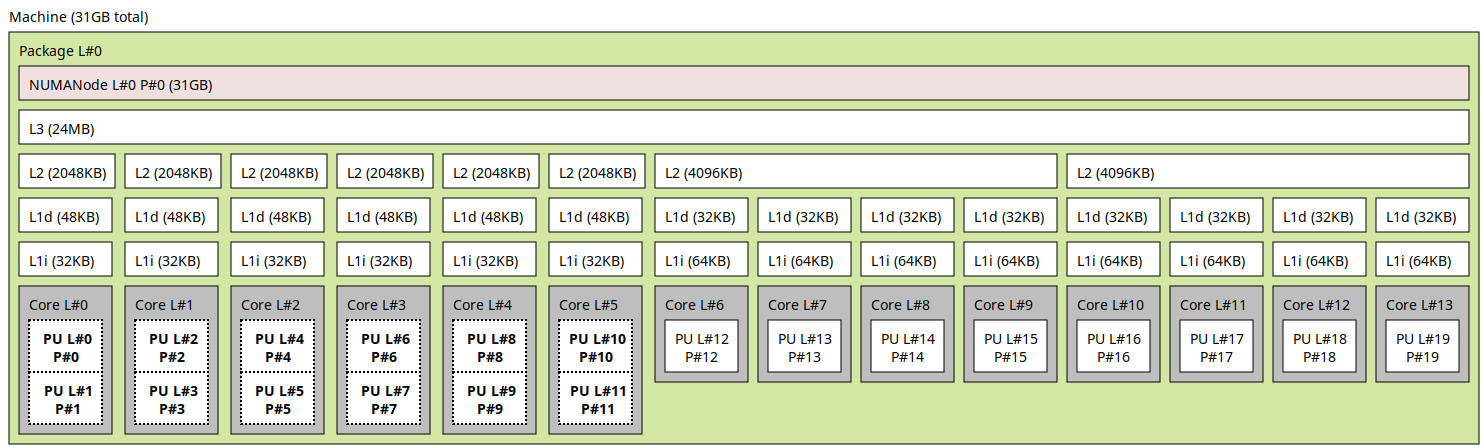
\includegraphics[width=0.8\textwidth]{lstopo.png}
    \caption{Output of lstopo}
\end{figure}

Since the target is an Intel i5-13600K it was determined to use a chunk size of 1MB. This would fit in the L2
cache of the P-cores, and E-cores of the device. There would be parts of a chunk evicted from cache or not loaded 
as other objects such as the Frequency object were still large, however this reduced the queue contention and
improved the performance of the application. The application CPU utilisation after the change of the chunk size
was between 1850\% and 1980\%. This was a significant improvement over the previous 800\%.

\subsection{Branch prediction}

The application was then profiled with Intel Advisor again. It was found that the transformation step was 
performing many memory operations. To make the algorithm more intense arithmetically it was determined that
the branch prediction needed to be improved.

Whenever a transformation occurs on a chunk of data, the existing pair is replaced with a new symbol and a 
symbol that represents a skip token. So when performing subsequent transformation there was a branch that 
checked if the current symbol was the skip token. As the program ran longer the skip token became more common.
This lead to a slowdown on subsequent iterations of the transformation step. 

To solve this during the transformation, step memory was moved so the significant tokens were contiguous. This 
lead to 20\% improvement in total program execution time for vocabularies $> 300$ tokens long.

Since this operation was fused into the transformation step it was also executed in parallel. This resulted in 
insignificant slowdown for very small vocabularies but a significant speedup for larger vocabularies. 

The improvement in branch prediction also lead to the count\_pairs function to become scalar addition bound on
the Intel Advisor roofline analysis.


\section{Explaination of the code}

As the entire application has been rewritten a revised class diagram has been created.

\begin{figure}[H]
    \centering
    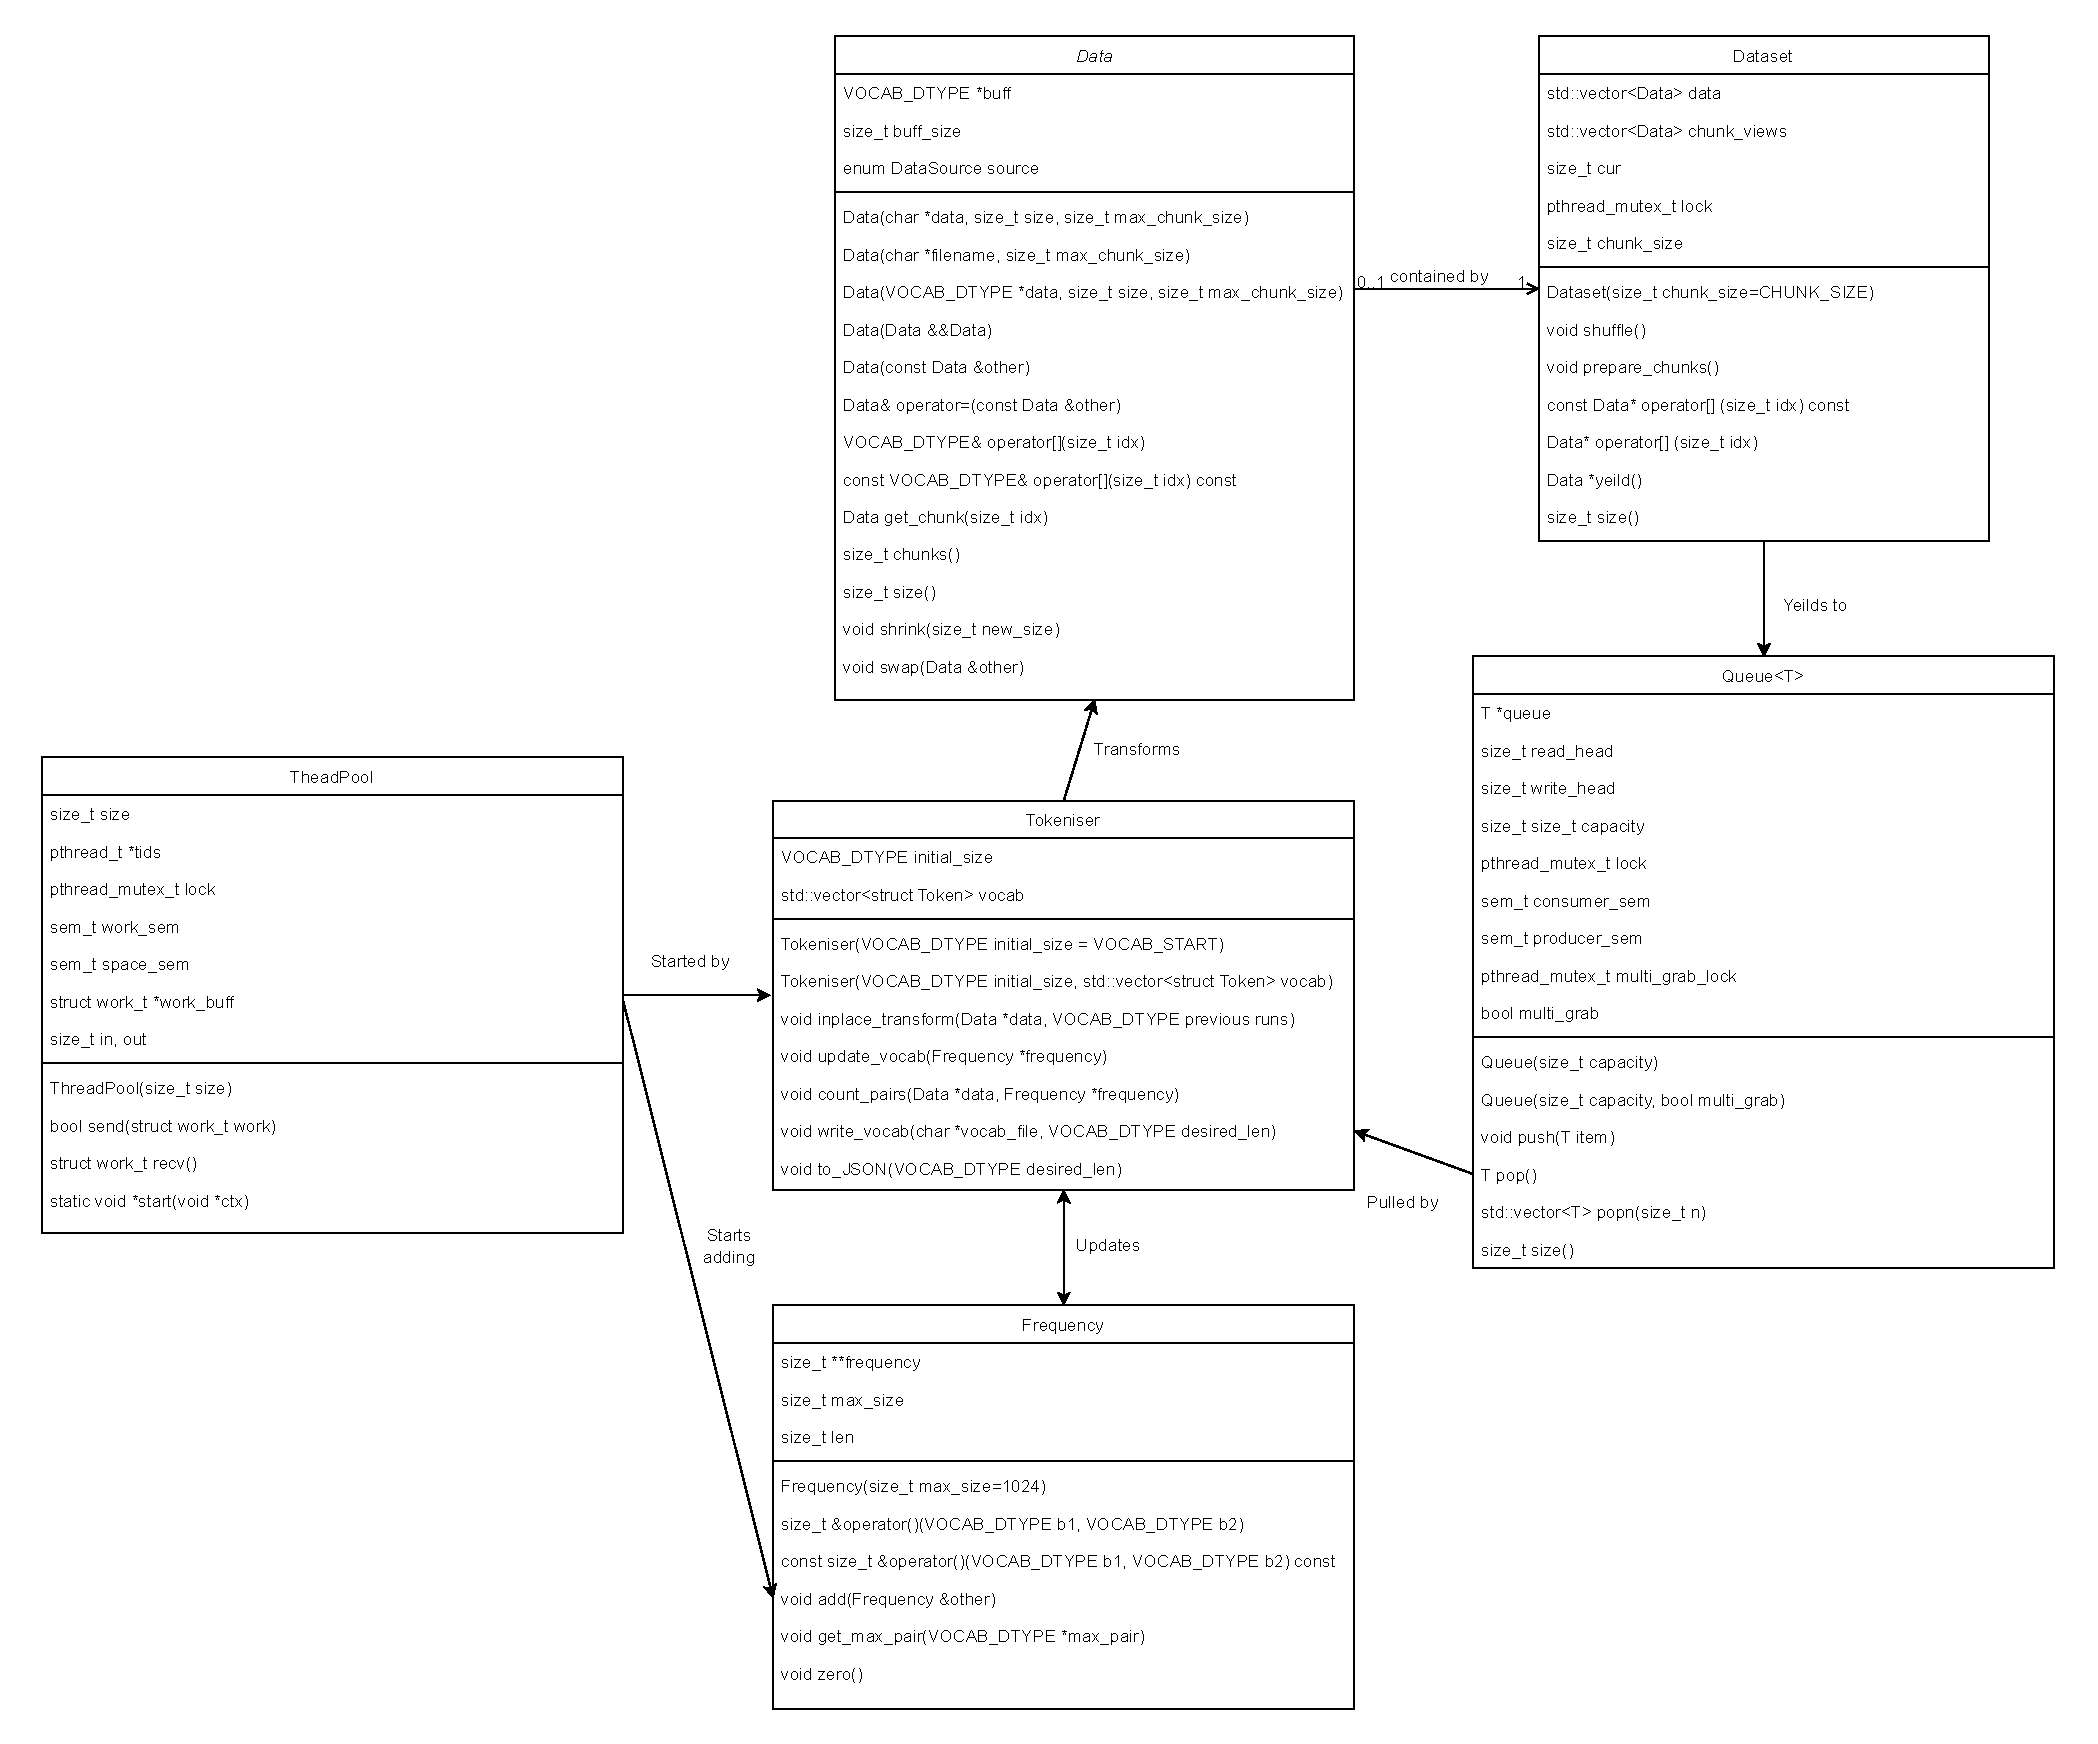
\includegraphics[width=0.6\textwidth]{class_diagram.pdf}
    \caption{Class diagram of the parallel application}
\end{figure}

As the application uses classes but is not entirely object oriented there are some functions missing in the diagram.
These functions are the main, status, train, transform\_worker count\_pairs\_worker, and sum\_worker functions. 
The main function chooses between the vocab training mode, and the status mode. The train function coordinates
the worker threads and the data flow for training a vocabulary. It passes the worker functions along with their 
arguments to the thread pool in the appropriate order.

As the program used to be a single line file the line counts of everything has changed. On a project level
the reference implementation was 353 lines long, and the parallel implementation is 1453 lines long.

\subsection{main.cpp (353 lines to 50 lines)}
The body of the main function is shown below. It initialises the thread pool, as it is used throughout the
application. It then parses the command line arguments and chooses the appropriate mode to run the application 
in. See appendix \ref{appendix:main} for the full code.


\subsection{queue.hpp (0 lines to 100 lines)}
As Queue is a templated class, the implementation is a single header file. When a queue is created the programmer 
can choose if the queue is capable of grabbing multiple items at once or not. If the queue is capable of doing this 
there is some extra synchronisation that allows only one thread to wait on the consumer semaphore at once. This is
implemented using a mutex. 

The most interesting functions are the \textit{push}, \textit{pop}, and \textit{popn} functions.

\begin{multicols}{2}
\begin{minted}{cpp}
template <typename T>
void Queue<T>::push(T item) { //Blocking
    sem_wait(&this->producer_sem);
    pthread_mutex_lock(&this->lock);
    
    queue[write_head] = item;
    write_head = (write_head + 1) % capacity;
    
    pthread_mutex_unlock(&this->lock);
    sem_post(&this->consumer_sem);
}
\end{minted} 

\begin{minted}{cpp}
    template <typename T>
    std::vector<T> Queue<T>::popn(size_t n) {
        if(!multi_grab) {
            throw std::runtime_error(
                "Multi grab not enabled");
        }
        pthread_mutex_lock(&this->multi_grab_lock);
        std::vector<T> items;
        for(size_t i = 0; i < n; i++) {
            items.push_back(pop());
        }
        pthread_mutex_unlock(&this->multi_grab_lock);
        return items;
    }
    \end{minted}

\begin{minted}{cpp}
template <typename T>
T Queue<T>::pop() { //Blocking
    if(!multi_grab) {
        pthread_mutex_lock(&this->multi_grab_lock);
    }
    
    sem_wait(&this->consumer_sem);
    pthread_mutex_lock(&this->lock);

    T item = queue[read_head];
    read_head = (read_head + 1) % capacity;

    pthread_mutex_unlock(&this->lock);
    sem_post(&this->producer_sem);

    if(!multi_grab) {
        pthread_mutex_unlock(&this->multi_grab_lock);
    }
    
    return item;
}
\end{minted}
\end{multicols}

\subsection{threadpool.hpp (0 lines to 124 lines)}
The thread pool is a class that takes a number of threads in the constructor and launches each thread to a
static member function in the class. It passes a pointer of itself to the function so the thread can pull 
from the queue. The functions of interest here are the send, recv, and start functions.

\begin{multicols}{2}

\begin{minted}{cpp}
bool ThreadPool::send(struct work_t work) {
    sem_wait(&(this->space_sem));

    //Just a push to the queue really
    pthread_mutex_lock(&this->lock);
    size_t next_in = (this->in + 1) % QUEUE_SIZE;
    if(next_in == this->out) { //There is no space to append
    //Really shouldn't ever happen because of the semaphore
        pthread_mutex_unlock(&(this->lock)); 
        sem_post(&(this->space_sem));
        return false;
    }

    this->work_buff[this->in] = work;
    this->in = next_in;

    pthread_mutex_unlock(&this->lock);
    sem_post(&(this->work_sem));
    
    return true;
}
\end{minted}

\begin{minted}{cpp}
struct work_t ThreadPool::recv() {
    struct work_t work = {.fn = nullptr, .data=nullptr};
    
    sem_wait(&(this->work_sem));
    pthread_mutex_lock(&(this->lock));

    work = this->work_buff[this->out];
    this->out = (this->out + 1) % QUEUE_SIZE;

    pthread_mutex_unlock(&this->lock);
    sem_post(&(this->space_sem));

    return work;
}
\end{minted}

\begin{minted}{cpp}
void* ThreadPool::start(void *ctx) {
    ThreadPool *pool = (ThreadPool *)ctx;
    while(true) {
        struct work_t work = pool->recv();
        if(work.fn == nullptr) {
            break;
        }
        work.fn(work.data);
    }
    return nullptr;
}
\end{minted}

\end{multicols}

\subsection{frequency.cpp (0 lines to 103 lines)}
The functtion of interest in the frequency class is how OpenMP SIMD was used when adding objects.

\begin{minted}{cpp}
void Frequency::add(Frequency &other) {
    for(size_t i = 0; i < this->max_size; i++) {
        if(this->frequency[i] == nullptr && other.frequency[i] == nullptr) {
            continue;
        }
        if(this->frequency[i] == nullptr) {
            this->frequency[i] = new size_t[this->max_size];
            memcpy(this->frequency[i], other.frequency[i], this->max_size * sizeof(size_t));
            continue;
        }
        if(other.frequency[i] == nullptr) {
            continue;
        }

        #pragma omp simd
        for(size_t j = 0; j < this->max_size; j++) {
            this->frequency[i][j] += other.frequency[i][j];
        }
    }
    return;
}
\end{minted}


\subsection{dataset.cpp (0 lines to 82 lines)}
The function of interest here is the function that gets the chunk views on each iteration of the training loop.
OpenMP was used to parallelise the loop with a critical section to prevent race conditions.

\begin{minted}{cpp}
void Dataset::prepare_chunks() {
    //Before executing this make sure the tokeniser has been run on the data
    pthread_mutex_lock(&this->lock);

    chunk_views.clear();
    #pragma omp parallel for
    for (size_t i = 0; i < data.size(); i++) {
        for (size_t j = 0; j < data[i].chunks(); j++) {
            Data chunk = data[i].get_chunk(j);
            #pragma omp critical
            this->chunk_views.push_back(chunk);
        }
    }
    this->cur = 0;

    pthread_mutex_unlock(&this->lock);
}
\end{minted}


\subsection{tokeniser.cpp (0 lines to 137 lines)}
The tokeniser class was designed such that all functions were thread safe, assuming they were not called on 
overlapping data, so the implementation does not change between the serial and parallel implementations. 
Since it is a complete rewrite and there is no parallelisation happening inside the functions it has been 
included in appendix \ref{appendix:tokeniser} for brevity.

\subsection{data.cpp (0 lines to 203 lines)}
The data class is just a container class to load the data and provide views of the data that modify the 
underlying data. There is no explicit parallelisation in these functions and they are threadsafe if called on 
non overlapping data. The implementation is included in appendix \ref{appendix:data} for brevity.

\subsection{equiavlence.py (0 lines to 12 lines)}
As the program has a file output a simple comparison of the output can be acheived with a small python script.

\begin{minted}{python}
parallel_filepath = open("parallel.vocab", "rb")
serial_filepath = open("serial.vocab", "rb")

parallel_output = parallel_filepath.read()
serial_output = serial_filepath.read()

if parallel_output == serial_output:
    print("The two implementations are equivalent")
else:
    print("The two implementations are not equivalent")
\end{minted}

\subsection{train.cpp (0 lines to 262 lines)}

There are a number of functions of interest in the train.cpp file, train, transform\_worker, train\_vocab\_worker,
and sum\_vocab\_worker.

\begin{minted}{cpp}
struct sum_vocab_arg {
    Queue<Frequency *> *queue;
    pthread_mutex_t *lock;
    sem_t *sums_finished;
    size_t *sums_occured;
    uint32_t target_sums;
};

void sum_vocab_worker(void *data) {
    struct sum_vocab_arg *arg_p = (struct sum_vocab_arg *)data;
    Queue<Frequency *> *queue = arg_p->queue;
    

    //Consume queue
    std::vector<Frequency *> frequencies = queue->popn(2);
    Frequency *lhs = frequencies[0];
    Frequency *rhs = frequencies[1];
    lhs->add(*rhs);
    queue->push(lhs);
    delete rhs;
    
    pthread_mutex_lock(arg_p->lock);
    (*arg_p->sums_occured)++;
    if(*arg_p->sums_occured == (size_t)arg_p->target_sums) {
        sem_post(arg_p->sums_finished);
    }
    pthread_mutex_unlock(arg_p->lock);

    free(arg_p);
    return;
}
\end{minted}

\begin{minted}{cpp}
struct train_msg_t {
    enum msg_type type;
    Data *data;
};

struct train_arg {
    Queue<struct train_msg_t> *queue;
    Queue<Frequency *> *reply;
    VOCAB_DTYPE current_vocab_size;
    VOCAB_DTYPE initial_size_of_vocab;
    std::vector<struct Token> *vocab;
};

void train_vocab_worker(void *data) {
    struct train_arg *arg_p = (struct train_arg* )data;
    
    VOCAB_DTYPE current_vocab_size = arg_p->current_vocab_size;
    Queue<struct train_msg_t> *queue = arg_p->queue;
    Queue<Frequency *> *reply = arg_p->reply;
    Tokeniser tokeniser(arg_p->initial_size_of_vocab, *arg_p->vocab);

    free(arg_p);

    Frequency *frequency_p = new Frequency(current_vocab_size); //Initialise the frequency object with the max size

    while(true) {
        struct train_msg_t msg = queue->pop();

        switch(msg.type) {
            case DATA:
                //tokeniser.inplace_transform(msg.data, current_vocab_size - VOCAB_START - 1);
                tokeniser.count_pairs(msg.data, frequency_p);
                break;
            case DATA_FIN:
                reply->push(frequency_p);
                
                return;
        }
    }
    free(arg_p);
    return;
}
\end{minted}

\begin{minted}{cpp}
struct transform_args_t {
    Tokeniser *tokeniser;
    Data *data;
    sem_t *transform_complete;
    VOCAB_DTYPE vocab_size;
    size_t *transforms;
    size_t total_tranforms;
    pthread_mutex_t *lock;
};

void transform_worker(void *arg) {
    struct transform_args_t *args = (struct transform_args_t *)arg;
    Tokeniser *tokeniser = args->tokeniser;
    Data *data = args->data;
    VOCAB_DTYPE vocab_size = args->vocab_size;

    if(vocab_size != 0) {
        tokeniser->inplace_transform(data, vocab_size-1); //Perform the transformation at the top of the stack
    }
    
    pthread_mutex_lock(args->lock);
    (*args->transforms)++;
    

    if(*(args->transforms) == args->total_tranforms) {
        sem_post(args->transform_complete);
    }
    pthread_mutex_unlock(args->lock);

    free(args);
    return;
}
\end{minted}

\begin{minted}{cpp}
//Initialize the dataset 
std::vector<char *> filepaths;
for(size_t i = 0; i < command_line_args.file_count; i++) {
    filepaths.push_back(command_line_args.filepaths[i]);
}
DatasetFiles dataset(CHUNK_SIZE, filepaths);

//Initialize the tokeniser
Tokeniser tokeniser(VOCAB_START);

//Training loops

for(size_t i = 0; i < command_line_args.vocab_size-VOCAB_START; i++) {
    sem_t transform_complete;
    sem_init(&transform_complete, 0, 0);

    pthread_mutex_t transform_lock;
    size_t transforms = 0;
    pthread_mutex_init(&transform_lock, nullptr);

    //Transform the underlying data in parallel
    size_t dataset_underlying_data_size = dataset.data.size();
    for(size_t j = 0; j < dataset_underlying_data_size; j++) {
        struct transform_args_t *args = (struct transform_args_t *)malloc(sizeof(struct transform_args_t));
        if(args == nullptr) {
            exit(150);
        }
        
        args->tokeniser=&tokeniser;
        args->data=&(dataset.data[j]); 
        args->transform_complete=&transform_complete;
        args->vocab_size=i;
        args->transforms=&transforms;
        args->total_tranforms=dataset_underlying_data_size;
        args->lock=&transform_lock;

        pool->send({.fn=transform_worker, .data=(void*)args});
    }

    sem_wait(&transform_complete);
    sem_destroy(&transform_complete);

    dataset.prepare_chunks();

    //Initialize the Queues
    Queue<struct train_msg_t> comms_queue(QUEUE_SIZE);
    Queue<Frequency *> reply_queue(QUEUE_SIZE, true);

    for(size_t j = 0; j < processor_count; j++) {
        struct train_arg *arg = (struct train_arg *)malloc(sizeof(struct train_arg));
        if(arg == nullptr) {
            exit(150);
        }

        arg->queue = &comms_queue;
        arg->reply = &reply_queue;
        arg->initial_size_of_vocab = VOCAB_START;
        arg->current_vocab_size = VOCAB_START + i;
        arg->vocab = &tokeniser.vocab;

        //
        struct work_t data = {.fn=train_vocab_worker, .data=(void*)arg};
        pool->send(data);
    }

    for(size_t j = 0; j < dataset.size(); j++) {
        Data *data = dataset.yeild(); 
        struct train_msg_t msg = {.type=DATA, .data=data};
        comms_queue.push(msg);
    }

    for(size_t j = 0; j < processor_count; j++) { //Send the request for the frequency object
        struct train_msg_t msg = {.type=DATA_FIN, .data=nullptr};
        comms_queue.push(msg);
    }

    //Receive them back
    size_t processed = 0;
    //Number of workers that have a frequency object that can be summed together to make the final frequency object
    size_t target_sums = processor_count-1; 

    //Set up the sum workers
    pthread_mutex_t sum_worker_lock;
    pthread_mutex_init(&sum_worker_lock, nullptr);

    sem_t sums_finished;
    sem_init(&sums_finished, 0, 0);

    for(size_t j = 0; j < target_sums; j++) {
        struct sum_vocab_arg *arg = (struct sum_vocab_arg *)malloc(sizeof(struct sum_vocab_arg));
        if(arg == nullptr) {
            exit(150);
        }
        

        arg->lock = &sum_worker_lock;
        arg->queue = &reply_queue;
        arg->sums_finished = &sums_finished;
        arg->sums_occured = &processed;
        arg->target_sums = target_sums;

        struct work_t data = {.fn=sum_vocab_worker, .data=(void*)arg};
        pool->send(data);
    }
    sem_wait(&sums_finished); //Flags when we are done
    printf("Finished token %lu\n", i + VOCAB_START);
    sem_destroy(&sums_finished);
    pthread_mutex_destroy(&sum_worker_lock);
    Frequency *frequencies = reply_queue.pop(); //Pop the final frequency object
    tokeniser.update_vocab(frequencies);
    delete frequencies;

    tokeniser.write_vocab(vocab_filename, command_line_args.vocab_size);
}
return 0;
\end{minted}

\section{Learnings}

There were many learnings from this project, cache locality, over synchronisation, 
value in over decomposition, branch prediction optimisation, OpenMP SIMD, patterns for pthreads work, 
and the power of perf and Intel Advisor. 

The most significant learning is in pthreads and how it can be used to allow for fine grained control over 
how data and work flows through a program across all platforms that support POSIX 2008. While OpenMP could 
be used for this there are ways to take advantage of the POSIX threading API that OpenMP does not provide.

OpenMP SIMD was noted for its ease of use and cross platform support and support for many architectures.
It is limited, as SIMD always is, to the type of operations that can be vectorised. The constant stride, 
lack of branching, and lack of memory dependencies are all required for SIMD to be effective.

Intel Advisor and perf were invaluable in finding room for optimisation, along with directing the priority
of optimisation. The roofline analysis was particularly useful in determining where the application was
constrained by data bandwidth or CPU compute, and if it was neither of these things for a integer or float 
operation heavy algorithm, then further investigation was required. 

The resulting project is quite an accomplishment, with many of the applications loops bounded by CPU compute
capability. The process leant throughout this project are highly applicable with machines becoming 
increasingly parallel, and it has been interesting to learn how to take advantage of these devices.

\section{References}
https://github.com/gcc-mirror/gcc/blob/1cb6c2eb3b8361d850be8e8270c597270a1a7967/libgomp/iter.c

\appendix
\section{Appendix}

\subsection{Counting byte pairs to summing frequencies}
\label{appendix:counting_to_summing}
\begin{minted}{C}
Queue<struct train_msg_t> comms_queue(QUEUE_SIZE);
Queue<Frequency *> reply_queue(QUEUE_SIZE, true);

for(size_t j = 0; j < processor_count; j++) {
    struct train_arg *arg = (struct train_arg *)malloc(sizeof(struct train_arg));
    if(arg == nullptr) {
        exit(150);
    }

    arg->queue = &comms_queue;
    arg->reply = &reply_queue;
    arg->initial_size_of_vocab = VOCAB_START;
    arg->current_vocab_size = VOCAB_START + i;
    arg->vocab = &tokeniser.vocab;

    //
    struct work_t data = {.fn=train_vocab_worker, .data=(void*)arg};
    pool->send(data);
}

for(size_t j = 0; j < dataset.size(); j++) {
    Data *data = dataset.yeild(); //FIXME if this goes out of scope before being processed it is a use after free
    struct train_msg_t msg = {.type=DATA, .data=data};
    comms_queue.push(msg);
}

for(size_t j = 0; j < processor_count; j++) { //Send the request for the frequency object
    struct train_msg_t msg = {.type=DATA_FIN, .data=nullptr};
    comms_queue.push(msg);
}

//Receive them back
size_t processed = 0;
size_t target_sums = processor_count-1; //Number of workers that have a frequency object that can be summed together to make the final frequency object

//Set up the sum workers
pthread_mutex_t sum_worker_lock;
pthread_mutex_init(&sum_worker_lock, nullptr);

sem_t sums_finished;
sem_init(&sums_finished, 0, 0);

for(size_t j = 0; j < target_sums; j++) {
    struct sum_vocab_arg *arg = (struct sum_vocab_arg *)malloc(sizeof(struct sum_vocab_arg));
    if(arg == nullptr) {
        exit(150);
    }
    

    arg->lock = &sum_worker_lock;
    arg->queue = &reply_queue;
    arg->sums_finished = &sums_finished;
    arg->sums_occured = &processed;
    arg->target_sums = target_sums;

    struct work_t data = {.fn=sum_vocab_worker, .data=(void*)arg};
    pool->send(data);
}
sem_wait(&sums_finished); //Flags when we are done
printf("Finished token %lu\n", i + VOCAB_START);
sem_destroy(&sums_finished);
pthread_mutex_destroy(&sum_worker_lock);
Frequency *frequencies = reply_queue.pop(); //Pop the final frequency object
\end{minted}

\subsection{main.cpp}
\label{appendix:main}
\begin{minted}{cpp}
    const uint32_t processor_count = 20;//std::thread::hardware_concurrency();
    ThreadPool *pool = new ThreadPool(processor_count);
    
    struct command_line_args command_line_args;
    if(parse_argv(--argc, ++argv, &command_line_args)) {
        exit(2); //Error already printed in the parse_argv function;
    }
    
    switch(command_line_args.mode) {
        case MODE_TRAIN:
            train(command_line_args, processor_count, pool);
            break;
        case MODE_STATUS:
            return status(command_line_args);
            break;
        default:
            fprintf(stderr, "Bad mode\n");
            break;
    }
    \end{minted}

\end{document}